\pdfminorversion=6
\ifx\fhformat\undefined\def\fhformat{}\fi
\PassOptionsToPackage{english}{babel}
\documentclass[\fhformat,10pt]{fh-ooe}

\usepackage{bookmark}

% English metadata and language override the shared German deck defaults.
\selectlanguage{english}
\AtBeginDocument{\selectlanguage{english}}
\title[DACHS 2026]{\Huge Collaborative AI-Assisted Software Development in Teaching\\[0.35em]\Large using OpenAI Codex as an example}
\institute[FH Upper Austria -- Hagenberg]{FH Upper Austria -- Campus Hagenberg\\Department of Digital Media}
\date[07.09.2026]{7 September 2026}

% Key project and component references
\newcommand{\SNodeCLink}{\href{https://github.com/SNodeC/snode.c}{SNode.C}}
\newcommand{\AISuiteLink}{\href{https://github.com/SNodeC/AISuite}{AISuite}}
\newcommand{\CodexBridgeLink}{\href{https://github.com/SNodeC/AISuite}{\texttt{codex-bridge}}}
\newcommand{\CodexUILink}{\href{https://github.com/SNodeC/CodexUI}{CodexUI}}
\newcommand{\CodexWUILink}{\href{https://github.com/SNodeC/CodexUI}{CodexWUI}}
\newcommand{\CodexLink}{\href{https://github.com/openai/codex}{OpenAI Codex}}
\newcommand{\MQTTSuiteLink}{\href{https://github.com/SNodeC/mqttsuite}{MQTTSuite}}

\begin{document}

% 1: title page generated automatically by fh-ooe.cls

% -----------------------------------------------------------------------------
% 2
\section{I just wanted to use Codex effectively}
\begin{frame}{I just wanted to use Codex effectively}
\begin{columns}[T]
\column{0.46\textwidth}
\centering
\vspace{0.75em}
\begin{tikzpicture}[font=\small,>=Latex]
\node[draw,rounded corners,fill=dachslight,minimum width=3.2cm,minimum height=0.9cm] (codex) at (0,1.25) {\CodexLink};
\node (web) at (-2.0,-0.15) {Web};
\node (cli) at (0,-0.15) {CLI};
\node (ide) at (2.0,-0.15) {VS Code/JetBrains};
\draw[->,thick] (codex) -- (web);
\draw[->,thick,fh-ooe-red] (codex) -- (cli);
\draw[->,thick] (codex) -- (ide);
\end{tikzpicture}
\column{0.50\textwidth}
\begin{block}{My starting point}
\begin{itemize}
  \item I have been developing my own C++ networking framework for about seven years.
  \item I want to use Codex directly in my actual local workspace.
  \item My development environments are \textbf{Qt Creator} and \textbf{KDevelop}, rather than VS Code or JetBrains.
\end{itemize}
\end{block}
\vspace{0.25em}
\begin{alertblock}{Requirement}
The repository, compiler, build system, tests, Git and tools should stay \textbf{on my machine}.
\end{alertblock}
\end{columns}
\end{frame}

% -----------------------------------------------------------------------------
% 3
\section{The SNode.C networking framework in 60 seconds}
\begin{frame}{The SNode.C networking framework in 60 seconds}
\small
\begin{columns}[T]
\column{0.48\textwidth}
\begin{block}{General-purpose networking framework}
\begin{itemize}
  \item \SNodeCLink: C++20, lightweight, event-driven and layered
  \item for general networking and distributed applications
  \item particular focus: M2M and the Internet of Things
\end{itemize}
\end{block}
\begin{block}{Application protocols}
HTTP/HTTPS with an Express-like API, WebSocket/WSS, MQTT and MQTT over WebSocket, using a common framework model.
\end{block}
\column{0.48\textwidth}
\begin{block}{Multi-Transport}
\begin{itemize}
  \item Unix Domain Sockets
  \item IPv4 and IPv6
  \item Bluetooth RFCOMM and L2CAP
  \item unencrypted and TLS-encrypted stream variants
\end{itemize}
\end{block}
\begin{block}{Configuration as part of the system}
The C++ API, command line and configuration files use the same instance/section model.
\end{block}
\end{columns}
\vspace{0.15em}
\begin{alertblock}{Relevant to this talk}
\SNodeCLink{} provides the \textbf{networking, transport and configuration foundation} on which \AISuiteLink{} is built. It does not provide the AI functionality itself.
\end{alertblock}
\end{frame}

% -----------------------------------------------------------------------------
% 4
\section{The web is convenient, but does not fit my workflow}
\begin{frame}{The web is convenient, but does not fit my workflow}
\begin{columns}[T]
\column{0.48\textwidth}
\begin{block}{Codex Web}
\begin{itemize}
  \item very convenient to access
  \item development and compilation largely in a cloud environment
  \item further removed from the state of my actual local toolchain
  \item noticeably slower for interactive development
\end{itemize}
\end{block}
\column{0.48\textwidth}
\begin{block}{My local development environment}
\begin{itemize}
  \item actual Git working copy
  \item CMake / Ninja / Compiler
  \item tests and sanitizers
  \item local tools and configuration
  \item direct control over the state
\end{itemize}
\end{block}
\end{columns}
\vspace{0.55em}
\begin{center}
\Large
\textbf{I do not want to bring my project to Codex.}\\[0.25em]
\color{fh-ooe-red}\textbf{I want to bring Codex to my project.}
\end{center}
\end{frame}

% -----------------------------------------------------------------------------
% 5
\section{The CLI solves almost exactly this problem}
\begin{frame}{The CLI solves almost exactly this problem}
\begin{columns}[T]
\column{0.52\textwidth}
\centering
\vspace{0.65em}
\begin{tikzpicture}[font=\small,>=Latex]
\node[draw,rounded corners,fill=fh-ooe-red!8,minimum width=2.7cm,minimum height=0.8cm] (cli) {Codex CLI};
\node[draw,rounded corners,fill=dachslight,below left=0.9cm and 0.15cm of cli] (src) {Source};
\node[draw,rounded corners,fill=dachslight,below=0.9cm of cli] (build) {Build};
\node[draw,rounded corners,fill=dachslight,below right=0.9cm and 0.15cm of cli] (tests) {Tests};
\node[draw,rounded corners,fill=dachslight,below=0.75cm of build] (git) {Git / local tools};
\draw[<->,thick] (cli) -- (src);
\draw[<->,thick] (cli) -- (build);
\draw[<->,thick] (cli) -- (tests);
\draw[<->,thick] (build) -- (git);
\end{tikzpicture}
\column{0.44\textwidth}
\small
\begin{block}{What works well}
\begin{itemize}
  \item local, direct workspace access
  \item shell, build, tests and Git
  \item full Codex functionality
\end{itemize}
\end{block}
\begin{block}{But in long sessions}
\begin{itemize}
  \item a large stream of text
  \item threads and turns are harder to follow
  \item tool activity mixed with conversation
  \item multiple contexts become hard to track
\end{itemize}
\end{block}
\end{columns}
\vspace{0.1em}
\begin{alertblock}{Motivation}
\small I wanted all of Codex, with \textbf{better visibility and interaction}.
\end{alertblock}
\end{frame}

% -----------------------------------------------------------------------------
% 6
\section{The key component: Codex app-server}
\begin{frame}{The key component: Codex app-server}
\centering
\begin{tikzpicture}[
  box/.style={draw,rounded corners,fill=dachslight,minimum width=2.2cm,minimum height=0.72cm,align=center},
  core/.style={draw,rounded corners,fill=fh-ooe-red!8,minimum width=3.8cm,minimum height=0.9cm,align=center},
  >=Latex,font=\small]
\node[box] (cli) at (-4.35,1.45) {CLI};
\node[box] (vscode) at (-1.45,1.45) {VS Code};
\node[box] (jb) at (1.45,1.45) {JetBrains};
\node[box] (custom) at (4.35,1.45) {custom clients};
\node[core] (server) at (0,-0.05) {\href{https://github.com/openai/codex}{Codex app-server}\\structured interface};
\node[core,minimum width=2.5cm] (codex) at (0,-1.7) {Codex};
\foreach \x in {cli,vscode,jb,custom} \draw[->,thick] (\x) -- (server);
\draw[<->,very thick,fh-ooe-red] (server) -- (codex);
\end{tikzpicture}
\vspace{0.25em}
\small
\begin{columns}[T]
\column{0.48\textwidth}
\begin{block}{Explicit work objects}
Threads, Turns, Items, History, Status, Interrupt/Resume
\end{block}
\column{0.48\textwidth}
\begin{block}{Explicit actions}
Tool calls, shell execution, requests, responses, approvals
\end{block}
\end{columns}
\vspace{0.05em}
\begin{alertblock}{Important}
The app-server remains the \textbf{semantic authority}. Its interface makes a custom integration practical.
\end{alertblock}
\end{frame}

% -----------------------------------------------------------------------------
% 7
\section{AISuite: an integration layer around the interface}
\begin{frame}{AISuite: an integration layer around the interface}
\centering
\begin{tikzpicture}[
  box/.style={draw,rounded corners,minimum height=0.82cm,align=center,fill=dachslight},
  >=Latex,font=\small]
\node[box,minimum width=7.4cm] (front) at (0,2.0) {\CodexUILink{} / \CodexWUILink{} / additional clients};
\node[box,minimum width=7.4cm,fill=fh-ooe-red!8] (bridge) at (0,0.45) {\AISuiteLink{} / \CodexBridgeLink};
\node[box,minimum width=4.3cm] (server) at (0,-1.15) {Codex app-server};
\draw[<->,very thick] (front) -- node[right]{frontend protocol} (bridge);
\draw[<->,very thick,fh-ooe-red] (bridge) -- node[right]{native JSON-RPC} (server);
\end{tikzpicture}
\vspace{0.2em}
\small
\begin{columns}[T]
\column{0.32\textwidth}
\begin{block}{Integration}
Process/provider integration, typing, lifecycle
\end{block}
\column{0.32\textwidth}
\begin{block}{Transport}
Unix, IP, WebSocket, TLS, Framing, Bounds
\end{block}
\column{0.32\textwidth}
\begin{block}{Routing}
Requests, responses, notifications, multiple frontends
\end{block}
\end{columns}
\end{frame}

% -----------------------------------------------------------------------------
% 8
\section{SNode.C: the existing technical foundation}
\begin{frame}{SNode.C: the existing technical foundation}
\begin{columns}[T]
\column{0.51\textwidth}
\centering
\begin{tikzpicture}[font=\small,>=Latex]
\node[draw,rounded corners,fill=fh-ooe-red!8,minimum width=4.5cm,minimum height=0.75cm] (app) {\AISuiteLink{} / \CodexBridgeLink};
\node[draw,rounded corners,fill=dachslight,minimum width=4.5cm,minimum height=0.75cm,below=0.42cm of app] (proto) {HTTP / WebSocket / TLS};
\node[draw,rounded corners,fill=dachslight,minimum width=4.5cm,minimum height=0.75cm,below=0.42cm of proto] (net) {Unix / IPv4 / IPv6};
\node[draw,rounded corners,fill=dachslight,minimum width=4.5cm,minimum height=0.75cm,below=0.42cm of net] (core) {\SNodeCLink{} -- event-driven C++20};
\draw[->,thick] (core) -- (net);
\draw[->,thick] (net) -- (proto);
\draw[->,thick] (proto) -- (app);
\end{tikzpicture}
\column{0.45\textwidth}
\small
\begin{block}{Why it matters here}
\begin{itemize}
  \item networking and transport foundation for AISuite
  \item long-lived bidirectional connections
  \item process and event integration
\end{itemize}
\end{block}
\begin{block}{An additional purpose}
AISuite and CodexUI/WUI also provide a realistic \textbf{stress test for SNode.C}.
\end{block}
\end{columns}
\vspace{0.2em}
\begin{center}
\small
Codex helps develop SNode.C, which in turn provides the infrastructure for using Codex.
\end{center}
\end{frame}

% -----------------------------------------------------------------------------
% 9
\section{Clear responsibilities without a second backend}
\begin{frame}{Clear responsibilities without a second backend}
\centering
\begin{tikzpicture}[
  layer/.style={draw,rounded corners,minimum width=10.0cm,minimum height=1.0cm,align=center},
  >=Latex,font=\small]
\node[layer,fill=fh-ooe-red!8] (server) at (0,1.85) {\textbf{Codex app-server}\\Threads · Turns · Items · semantic state};
\node[layer,fill=dachslight] (bridge) at (0,0.25) {\textbf{\AISuiteLink{} / codex-bridge}\\Transport · Routing · Connection and request correlation};
\node[layer,fill=white] (ui) at (0,-1.35) {\textbf{\CodexUILink{} / \CodexWUILink}\\Presentation · Interaction · Local UI behavior};
\draw[<->,thick] (server) -- (bridge);
\draw[<->,thick] (bridge) -- (ui);
\end{tikzpicture}
\vspace{0.4em}
\begin{alertblock}{Design decision}
\small AISuite keeps \textbf{no second semantic copy} of threads, turns or items. The app-server remains the source of truth.
\end{alertblock}
\end{frame}

% -----------------------------------------------------------------------------
% 10
\section{The complete runtime architecture}
\begin{frame}{The complete runtime architecture}
\centering
\begin{tikzpicture}[
  box/.style={draw,rounded corners,fill=dachslight,minimum width=3.0cm,minimum height=0.85cm,align=center},
  wide/.style={draw,rounded corners,fill=fh-ooe-red!8,minimum width=5.5cm,minimum height=0.9cm,align=center},
  >=Latex,font=\small]
\node[box] (native) at (-3.7,1.9) {CodexUI\\Qt 6};
\node[box] (web) at (0,1.9) {CodexWUI\\Browser};
\node[box] (other) at (3.7,1.9) {additional clients};
\node[wide] (bridge) at (0,0.25) {AISuite / codex-bridge};
\node[box,minimum width=4.0cm] (server) at (0,-1.5) {Codex app-server};
\node[box,minimum width=2.5cm] (codex) at (0,-3.15) {Codex};
\foreach \x in {native,web,other} \draw[<->,thick] (\x) -- (bridge);
\draw[<->,very thick,fh-ooe-red] (bridge) -- node[right]{JSON-RPC} (server);
\draw[<->,thick] (server) -- (codex);
\node[draw,dashed,rounded corners,fit=(native)(web)(other)(bridge),inner sep=0.25cm,label={[font=\scriptsize]left:SNode.C-based side}] {};
\end{tikzpicture}
\vspace{0.15em}
\begin{center}
\scriptsize Frontends can connect locally or over the network. The app-server retains ownership of Codex semantics.
\end{center}
\end{frame}

% -----------------------------------------------------------------------------
% 11
\section{Deployment: computing power where development happens}
\begin{frame}{Deployment: computing power where development happens}
\centering
\begin{tikzpicture}[
  host/.style={draw,rounded corners,minimum width=6.4cm,minimum height=4.8cm,fill=dachslight,align=center},
  box/.style={draw,rounded corners,minimum width=3.6cm,minimum height=0.75cm,fill=white,align=center},
  client/.style={draw,rounded corners,minimum width=3.0cm,minimum height=1.0cm,fill=white,align=center},
  >=Latex,font=\small]
\node[host] (dev) at (0,0.35) {};
\node[font=\small\bfseries] at (0,2.35) {powerful development machine};
\node[box,fill=fh-ooe-red!8] (bridge) at (0,1.35) {codex-bridge};
\node[box] (server) at (0,0) {Codex app-server};
\node[box] (workspace) at (0,-1.35) {Repository · Build · Tests · Tools};
\node[font=\tiny,text=dachsgray,align=center] at (0,-2.4) {Owned mode: app-server launched / owned / monitored via stdio\\External: Unix / IPv4 / IPv6 WebSocket supported, currently unencrypted};
\draw[->,thick] (bridge) -- node[right,font=\scriptsize]{Lifecycle} (server);
\draw[<->,thick] (server) -- (workspace);
\node[client] (native) at (-5.25,1.35) {user computer\\CodexUI};
\node[client] (web) at (5.25,1.35) {user computer\\CodexWUI};
\draw[<->,very thick,fh-ooe-red] (native) -- (bridge);
\draw[<->,very thick,fh-ooe-red] (web) -- (bridge);
\end{tikzpicture}
\vspace{0.2em}
\begin{alertblock}{Implication}
\small The user computer only runs the interface and needs little computing power. The repository, compiler, tests and Codex execution stay on the development machine.
\end{alertblock}
\end{frame}

% -----------------------------------------------------------------------------
% 12
\section{Connections, provider path and platform status}
\begin{frame}{Connections, provider path and platform status}
\footnotesize
\begin{columns}[T]
\column{0.49\textwidth}
\begin{block}{Frontend $\leftrightarrow$ codex-bridge}
\textbf{CodexUI}
\begin{itemize}
  \item Unix domain socket, IPv4 and IPv6
  \item WebSocket connections
  \item plain or protected with SSL/TLS
\end{itemize}
\textbf{CodexWUI}
\begin{itemize}
  \item IPv4 / IPv6 over WebSocket
  \item plain or SSL/TLS
  \item only a browser required on the client
\end{itemize}
\end{block}
\begin{block}{codex-bridge $\leftrightarrow$ app-server}
\begin{itemize}
  \item stdio in local owned mode
  \item Unix Domain Socket
  \item IPv4 / IPv6 over WebSocket
  \item \textbf{The app-server currently offers no TLS on these provider paths.}
\end{itemize}
\end{block}
\column{0.47\textwidth}
\begin{alertblock}{Context}
\begin{itemize}
  \item The lack of encryption is therefore \textbf{not a limitation of codex-bridge}.
  \item Run the bridge and app-server on the same trusted machine where possible.
  \item Remote separation over untrusted networks requires additional protection.
\end{itemize}
\end{alertblock}
\begin{block}{Current status}
The native \texttt{codex-bridge} and CodexUI binaries currently target \textbf{Linux}. CodexWUI runs in a browser.
\end{block}
\end{columns}
\end{frame}

% -----------------------------------------------------------------------------
% 13
\section{CodexUI: my original goal}
\begin{frame}{CodexUI: my original goal}
\begin{columns}[T]
\column{0.48\textwidth}
\begin{block}{Native user interface}
\begin{itemize}
  \item \CodexUILink{} built with Qt 6 Widgets
  \item for the local desktop workflow
  \item explicit navigation of threads and turns
  \item visible tool and shell activity
  \item live state beyond a terminal text stream
\end{itemize}
\end{block}
\column{0.48\textwidth}
\centering
\begin{tikzpicture}[font=\small,>=Latex]
\node[draw,rounded corners,fill=dachslight,minimum width=4.0cm,minimum height=0.95cm] (qt) {Qt GUI Thread};
\node[draw,rounded corners,fill=white,minimum width=4.0cm,minimum height=0.95cm,below=0.62cm of qt] (q) {typed bounded queues};
\node[draw,rounded corners,fill=fh-ooe-red!8,minimum width=4.0cm,minimum height=0.95cm,below=0.62cm of q] (net) {SNode.C Client Thread};
\draw[<->,thick] (qt) -- (q);
\draw[<->,thick] (q) -- (net);
\node[draw,rounded corners,fit=(qt)(q)(net),inner sep=0.28cm,label={[font=\small\bfseries]above:CodexUI}] {};
\end{tikzpicture}
\vspace{0.25em}
\begin{block}{A native UI, not a WebView wrapper}
\small The native UI and network path are deliberately separate, but share the same current working state.
\end{block}
\end{columns}
\end{frame}

% -----------------------------------------------------------------------------
% 14
\section{Two interfaces, one backend}
\begin{frame}{Two interfaces, one backend}
\begin{columns}[T]
\column{0.49\textwidth}
\centering
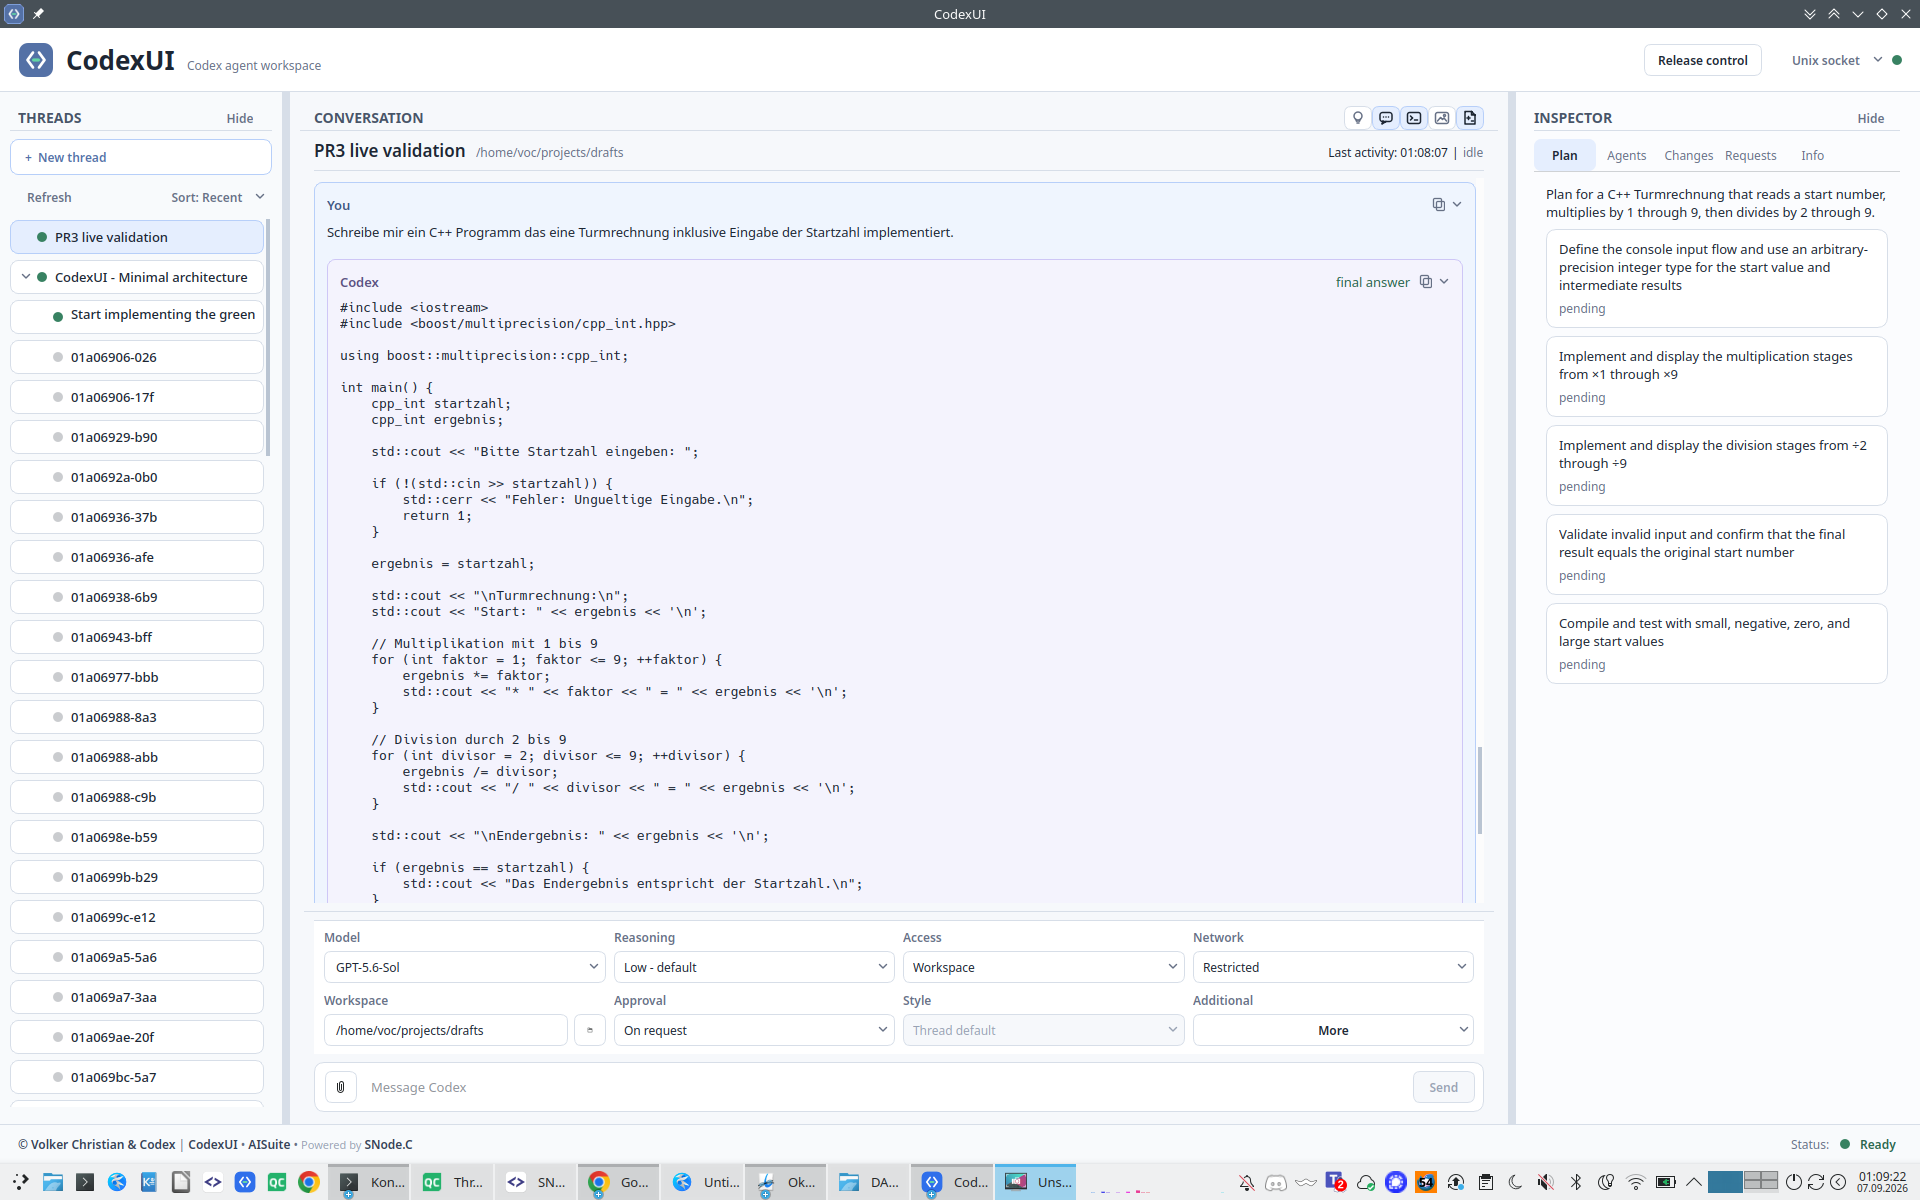
\includegraphics[width=0.96\linewidth,height=4.55cm,keepaspectratio]{screenshots/Screenshot_20260907_010922.png}
\\[0.4em]
\textbf{CodexUI -- native}
\column{0.49\textwidth}
\centering
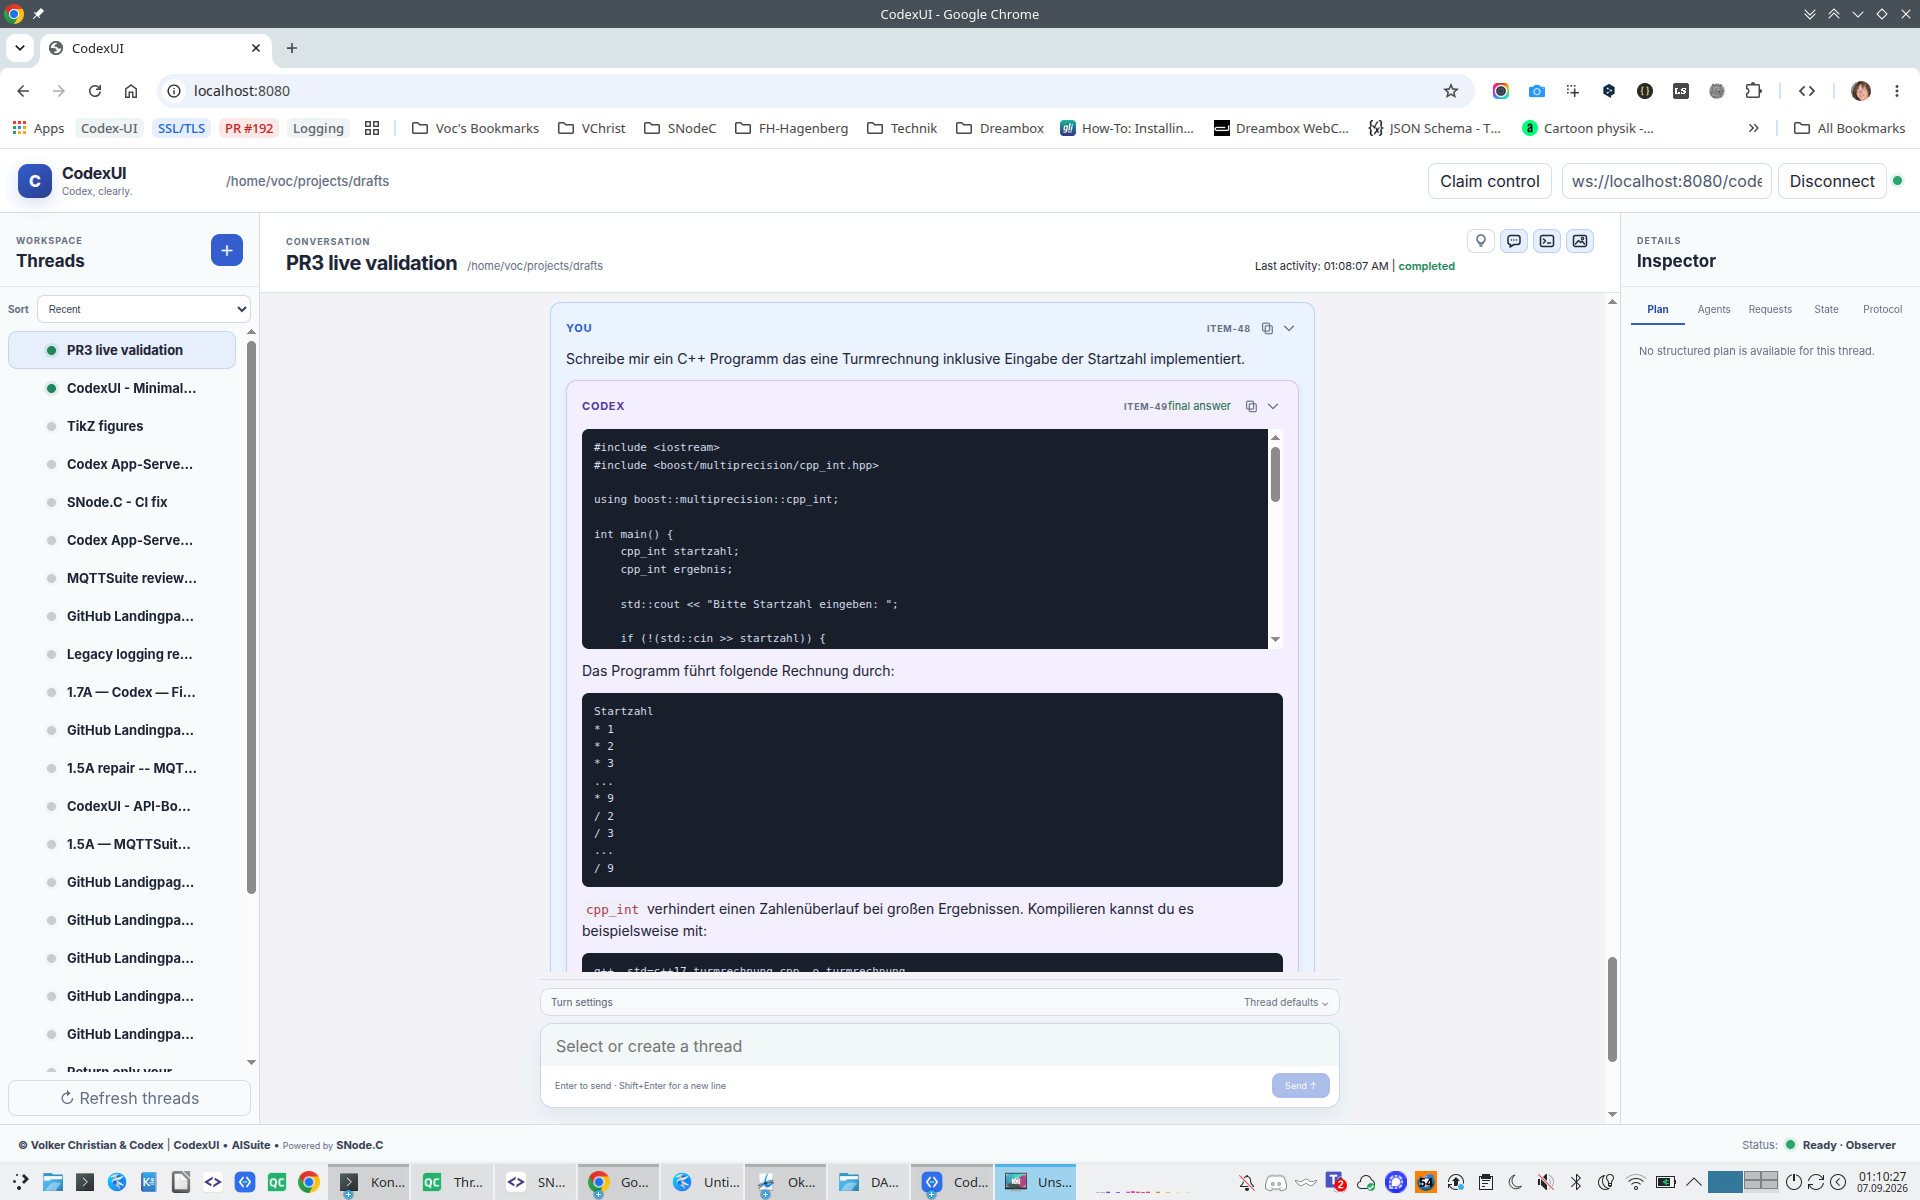
\includegraphics[width=0.96\linewidth,height=4.55cm,keepaspectratio]{screenshots/Screenshot_20260907_011027.png}
\\[0.4em]
\textbf{CodexWUI -- Web}
\end{columns}
\vspace{0.45em}
\begin{center}
\large
\textbf{Different presentation layers, the same app-server semantics.}
\end{center}
\end{frame}

% -----------------------------------------------------------------------------
% 15
\section{Why add a web version?}
\begin{frame}{Why add a web version?}
\begin{columns}[T]
\column{0.50\textwidth}
\centering
\begin{tikzpicture}[font=\small,>=Latex]
\node[draw,rounded corners,fill=dachslight,minimum width=3.1cm,minimum height=0.85cm] (native) at (-2.2,1.55) {CodexUI};
\node[draw,rounded corners,fill=dachslight,minimum width=3.1cm,minimum height=0.85cm] (web) at (2.2,1.55) {CodexWUI};
\node[draw,rounded corners,fill=fh-ooe-red!8,minimum width=4.3cm,minimum height=0.9cm] (bridge) at (0,-0.05) {codex-bridge};
\node[draw,rounded corners,fill=dachslight,minimum width=3.4cm,minimum height=0.85cm] (server) at (0,-1.65) {app-server};
\draw[<->,thick] (native) -- (bridge);
\draw[<->,thick] (web) -- (bridge);
\draw[<->,thick] (bridge) -- (server);
\end{tikzpicture}
\column{0.46\textwidth}
\small
\begin{block}{The browser changes access}
\begin{itemize}
  \item no local Qt installation required
  \item access from another machine
  \item the same backend
  \item the same threads and turns
  \item no separate AI backend
\end{itemize}
\end{block}
\begin{alertblock}{Implication}
The running engineering context becomes \textbf{accessible}, beyond a single interface.
\end{alertblock}
\end{columns}
\end{frame}

% -----------------------------------------------------------------------------
% 16
\section{The unexpected step: multiple clients}
\begin{frame}{The unexpected step: multiple clients}
\centering
\begin{tikzpicture}[
  client/.style={draw,rounded corners,fill=dachslight,minimum width=2.8cm,minimum height=0.8cm,align=center},
  core/.style={draw,rounded corners,fill=fh-ooe-red!8,minimum width=3.8cm,minimum height=0.9cm,align=center},
  >=Latex,font=\small]
\node[client] (c1) at (-4,1.8) {CodexUI};
\node[client] (c2) at (0,1.8) {CodexWUI};
\node[client] (c3) at (4,1.8) {another client};
\node[core] (bridge) at (0,0.2) {codex-bridge};
\node[client,minimum width=3.5cm] (server) at (0,-1.4) {one app-server context};
\foreach \x in {c1,c2,c3} \draw[<->,thick] (\x) -- (bridge);
\draw[<->,very thick,fh-ooe-red] (bridge) -- (server);
\end{tikzpicture}
\vspace{0.35em}
\begin{columns}[T]
\column{0.48\textwidth}
\begin{block}{Shared visibility}
\small Notifications, thread/turn progress, ongoing activity
\end{block}
\column{0.48\textwidth}
\begin{block}{Beyond a single screen}
\small Multiple frontends can follow the same engineering context.
\end{block}
\end{columns}
\end{frame}

% -----------------------------------------------------------------------------
% 17
\section{Collaboration needs explicit roles}
\begin{frame}{Collaboration needs explicit roles}
\begin{columns}[T]
\column{0.47\textwidth}
\centering
\begin{tikzpicture}[font=\small,>=Latex]
\node[draw,rounded corners,fill=fh-ooe-red!8,minimum width=2.5cm,minimum height=0.8cm] (ctrl) at (0,1.2) {Controller};
\node[draw,rounded corners,fill=dachslight,minimum width=2.3cm,minimum height=0.8cm] (o1) at (-2.3,0) {Observer};
\node[draw,rounded corners,fill=dachslight,minimum width=2.3cm,minimum height=0.8cm] (o2) at (2.3,0) {Observer};
\node[draw,rounded corners,fill=white,minimum width=3.7cm,minimum height=0.9cm] (bridge) at (0,-1.45) {codex-bridge};
\draw[<->,very thick,fh-ooe-red] (ctrl) -- (bridge);
\draw[<->,thick] (o1) -- (bridge);
\draw[<->,thick] (o2) -- (bridge);
\end{tikzpicture}
\column{0.49\textwidth}
\small
\begin{block}{Controller}
\begin{itemize}
  \item controls active requests
  \item answers relevant server-side requests
  \item currently holds input control
\end{itemize}
\end{block}
\begin{block}{Observer}
\begin{itemize}
  \item sees ongoing activity
  \item follows threads / turns / notifications
  \item does not change the state
\end{itemize}
\end{block}
\end{columns}
\vspace{0.1em}
\begin{alertblock}{Explicit handover}
\small Control changes hands deliberately. A disconnect does not silently promote another client to controller.
\end{alertblock}
\end{frame}

% -----------------------------------------------------------------------------
% 18
\section{Where this becomes useful for teaching}
\begin{frame}{Where this becomes useful for teaching}
\centering
\begin{tikzpicture}[
  box/.style={draw,rounded corners,minimum width=3.1cm,minimum height=0.8cm,align=center,fill=dachslight},
  >=Latex,font=\small]
\node[box] (code) at (-4.2,1.1) {Source code};
\node[box] (ctx) at (0,1.1) {AI working context};
\node[box] (tools) at (4.2,1.1) {Executed tools};
\node[box,fill=fh-ooe-red!8,minimum width=5.0cm] (process) at (0,-0.7) {shared engineering process};
\draw[->,thick] (code) -- (process);
\draw[->,thick] (ctx) -- (process);
\draw[->,thick] (tools) -- (process);
\end{tikzpicture}
\vspace{0.5em}
\begin{block}{A broader shared focus}
\small Teachers and students can observe the same ongoing AI-assisted engineering process and participate with explicit control, beyond viewing the results in the repository.
\end{block}
\end{frame}

% -----------------------------------------------------------------------------
% 19
\section{Three possible teaching scenarios}
\begin{frame}{Three possible teaching scenarios}
\small
\begin{columns}[T]
\column{0.32\textwidth}
\centering
\textbf{A -- Shared session}\\[0.3em]
\begin{tikzpicture}[font=\scriptsize,>=Latex]
\path[use as bounding box] (-1.7,-1.25) rectangle (1.7,1.55);
\node[draw,circle] (l) at (0,1.25) {T};
\node[draw,circle] (s1) at (-1.05,0.15) {S1};
\node[draw,circle] (s2) at (1.05,0.15) {S2};
\node[draw,rounded corners,fill=dachslight,minimum width=2.5cm] (b) at (0,-1.0) {one session};
\foreach \x in {l,s1,s2} \draw[<->] (\x) -- (b);
\end{tikzpicture}
\\[0.05em]
\scriptsize Debugging, architecture, review

\column{0.34\textwidth}
\centering
\textbf{B -- Individual sessions}\\[0.3em]
\begin{tikzpicture}[font=\tiny,>=Latex,
  session/.style={draw,rounded corners,fill=dachslight,minimum width=1.3cm,minimum height=1.05cm,align=center}]
\path[use as bounding box] (-1.7,-1.25) rectangle (1.7,1.55);
\node[draw,circle] (l) at (0,1.35) {T};
\node[session] (s1) at (-1.35,-0.35) {S1\\own\\session};
\node[session,fill=fh-ooe-red!8] (s2) at (0,-0.35) {S2\\own\\session};
\node[session] (s3) at (1.35,-0.35) {S3\\own\\session};
\draw[<->,thin] (l) -- (s1);
\draw[<->,very thick,fh-ooe-red] (l) -- (s2);
\draw[<->,thin] (l) -- (s3);
\end{tikzpicture}
\\[0.05em]
\scriptsize targeted support for an individual session

\column{0.30\textwidth}
\centering
\textbf{C -- Switching roles}\\[0.3em]
\begin{tikzpicture}[font=\scriptsize,>=Latex]
\path[use as bounding box] (-1.7,-1.25) rectangle (1.7,1.55);
\node[draw,rounded corners,fill=dachslight] (a) at (-1.15,0.8) {A};
\node[draw,rounded corners,fill=dachslight] (b) at (1.15,0.8) {B};
\node[draw,rounded corners,fill=fh-ooe-red!8,minimum width=2.45cm] (w) at (0,-0.75) {shared context};
\draw[->,thick] (a) -- node[left]{Implementation} (w);
\draw[->,thick,fh-ooe-red] (b) -- node[right]{Review} (w);
\end{tikzpicture}
\\[0.05em]
\scriptsize Peer review / handover
\end{columns}
\vspace{0.2em}
\begin{center}
\scriptsize\textbf{Key:} T = Teacher \qquad S = Student\\[0.2em]
\scriptsize\textbf{And any useful combination of these three basic scenarios.}
\end{center}
\vspace{0.05em}
\begin{alertblock}{What is new}
\small The new element is \textbf{AI-assisted engineering sessions that participants can observe together and hand over}, rather than ``AI as a tutor''.
\end{alertblock}
\end{frame}

% -----------------------------------------------------------------------------
% 20
\section{Live demo: the same session, two clients}
\begin{frame}{Live demo: the same session, two clients}
\centering
\begin{tikzpicture}[
  box/.style={draw,rounded corners,fill=dachslight,minimum width=3.0cm,minimum height=0.82cm,align=center},
  >=Latex,font=\small]
\node[box] (native) at (-3.2,1.75) {CodexUI\\local};
\node[box] (web) at (3.2,1.75) {CodexWUI\\Browser};
\node[box,fill=fh-ooe-red!8,minimum width=4.2cm] (bridge) at (0,0.15) {codex-bridge};
\node[box] (server) at (0,-1.3) {app-server};
\node[box] (codex) at (0,-2.75) {Codex};
\draw[<->,thick] (native) -- (bridge);
\draw[<->,thick] (web) -- (bridge);
\draw[<->,thick] (bridge) -- (server);
\draw[<->,thick] (server) -- (codex);
\end{tikzpicture}
\vspace{0.2em}
\small
\begin{columns}[T]
\column{0.49\textwidth}
\begin{enumerate}
  \item analyse a small, real C++ task
  \item make a change / run a test locally
\end{enumerate}
\column{0.49\textwidth}
\begin{enumerate}
  \setcounter{enumi}{2}
  \item connect the WUI to the same context
  \item brief role switch / review
\end{enumerate}
\end{columns}
\vspace{0.05em}
\begin{center}\scriptsize Goal: \textbf{demonstrate the architecture}, rather than tour the features.\end{center}
\end{frame}

% -----------------------------------------------------------------------------
% 21
\section{What it has become}
\begin{frame}{What it has become}
\centering
\begin{tikzpicture}[font=\scriptsize,>=Latex,node distance=0.34cm]
\tikzset{phase/.style={draw,rounded corners,fill=dachslight,minimum height=0.82cm,align=center,inner ysep=0pt,font=\small,text height=1.5ex,text depth=0.35ex}}
\node[phase,minimum width=2.65cm] (p1) {local Codex workflow};
\node[phase,minimum width=2.05cm,right=of p1] (p2) {app-server};
\node[phase,minimum width=1.85cm,right=of p2,fill=fh-ooe-red!8] (p3) {AISuite};
\node[phase,minimum width=2.15cm,right=of p3] (p4) {CodexUI/WUI};
\node[phase,minimum width=1.95cm,right=of p4] (p5) {Multi-Client};
\foreach \a/\b in {p1/p2,p2/p3,p3/p4,p4/p5} \draw[->,thick] (\a) -- (\b);
\end{tikzpicture}
\vspace{0.3em}
\small
\begin{columns}[T]
\column{0.48\textwidth}
\begin{block}{Result}
\begin{itemize}
  \item CodexUI is mature enough for \textbf{complex real-world projects}.
  \item Multiple clients extend a personal assistant into a \textbf{collaborative engineering workspace}.
  \item Codex semantics, integration and presentation remain clearly separated in the architecture.
\end{itemize}
\end{block}
\column{0.48\textwidth}
\begin{block}{How it was developed}
\begin{itemize}
  \item \textbf{Not a single line of project code was written by hand.}
  \item Codex implements AISuite, CodexUI and CodexWUI. \textbf{My role is the architect's}: requirements, architecture, review and direction.
  \item SNode.C supports a system that in turn helps \textbf{develop SNode.C further}.
\end{itemize}
\end{block}
\end{columns}
\end{frame}

% -----------------------------------------------------------------------------
% 22
\section{Outlook: additional AI providers for AISuite}
\begin{frame}{Outlook: additional AI providers for AISuite}
\centering
\begin{tikzpicture}[
  box/.style={draw,rounded corners,minimum height=0.85cm,align=center,fill=dachslight},
  provider/.style={draw,dashed,rounded corners,minimum width=3.0cm,minimum height=1.0cm,align=center,fill=white},
  >=Latex,font=\small]
\node[box,minimum width=7.2cm] (front) at (0,2.0) {CodexUI / CodexWUI / additional clients};
\node[box,fill=fh-ooe-red!8,minimum width=7.2cm] (suite) at (0,0.55) {AISuite\\shared integration and transport layer};
\node[provider,solid] (codex) at (-4.0,-1.35) {OpenAI Codex\\app-server};
\node[provider] (claude) at (0,-1.35) {Claude Code\\provider adapter};
\node[provider] (future) at (4.0,-1.35) {additional AI providers\\future option};
\draw[<->,thick] (front) -- (suite);
\draw[<->,thick] (suite) -- (codex);
\draw[<->,thick] (suite) -- (claude);
\draw[<->,thick] (suite) -- (future);
\end{tikzpicture}
\vspace{0.35em}
\small
\begin{columns}[T]
\column{0.48\textwidth}
\begin{block}{Goal}
Provider-specific protocols and lifecycles are encapsulated behind a common AISuite abstraction.
\end{block}
\column{0.48\textwidth}
\begin{block}{Implication}
Frontend, transport and collaboration concepts should remain reusable with other coding agents.
\end{block}
\end{columns}
\begin{center}
\scriptsize Claude Code and other providers are explicitly \textbf{future directions}, not the current implementation.
\end{center}
\end{frame}

% -----------------------------------------------------------------------------
% 23
\section{Outlook: from workspace to orchestrator}
\begin{frame}{Outlook: from workspace to orchestrator}
\centering
\begin{tikzpicture}[
  orch/.style={draw,rounded corners,fill=fh-ooe-red!8,minimum width=4.6cm,minimum height=0.95cm,align=center},
  session/.style={draw,rounded corners,fill=dachslight,minimum width=3.0cm,minimum height=1.25cm,align=center},
  >=Latex,font=\scriptsize]
\node[orch] (ui) at (0,2.25) {CodexUI / CodexWUI\\Session orchestration};
\node[session] (s1) at (-4.1,-0.15) {Machine A\\codex-bridge + app-server\\\texttt{CODEX\_HOME A}};
\node[session] (s2) at (0,-0.15) {Machine A\\codex-bridge + app-server\\\texttt{CODEX\_HOME B}};
\node[session] (s3) at (4.1,-0.15) {Machine B\\codex-bridge + app-server\\\texttt{CODEX\_HOME C}};
\draw[<->,thick] (ui) -- (s1);
\draw[<->,thick] (ui) -- (s2);
\draw[<->,thick] (ui) -- (s3);
\node[below=0.25cm of s1,text=dachsgray] {separate history / context};
\node[below=0.25cm of s2,text=dachsgray] {separate history / context};
\node[below=0.25cm of s3,text=dachsgray] {separate history / context};
\end{tikzpicture}
%\vspace{0.5em}
\small
\begin{columns}[T]
\column{0.32\textwidth}
\begin{block}{Independent sessions}
Multiple app-server instances with separate context/history directories.
\end{block}
\column{0.32\textwidth}
\begin{block}{Distributed machines}
Workspaces and toolchains can reside where they are actually needed.
\end{block}
\column{0.32\textwidth}
\begin{block}{Orchestration}
CodexUI/WUI manages selection and switching across many sessions, with roles as a future extension.
\end{block}
\end{columns}
\end{frame}

% -----------------------------------------------------------------------------
% 24
\section{References and projects}
\begin{frame}{References and projects}
\small
\begin{itemize}
  \item \textbf{\href{https://github.com/openai/codex}{OpenAI Codex CLI}} -- local coding agent with direct access to the workspace, shell, build, tests and Git.\\[-0.05em]
        \href{https://github.com/openai/codex}{\texttt{github.com/openai/codex}}
  \item \textbf{\href{https://github.com/openai/codex}{Codex app-server}} -- structured programming interface to Codex with threads, turns, items, tool calls and notifications.\\[-0.05em]
        \href{https://github.com/openai/codex}{\texttt{github.com/openai/codex}}
  \item \textbf{\SNodeCLink} -- general-purpose, event-driven C++20 networking framework and the technical foundation of this integration.\\[-0.05em]
        \href{https://github.com/SNodeC/snode.c}{\texttt{github.com/SNodeC/snode.c}}
  \item \textbf{\AISuiteLink{} / \CodexBridgeLink} -- AI integration layer with provider connections, transport, routing and support for multiple clients.\\[-0.05em]
        \href{https://github.com/SNodeC/AISuite}{\texttt{github.com/SNodeC/AISuite}}
  \item \textbf{\CodexUILink{} / \CodexWUILink} -- native Qt 6 and browser-based frontends for AISuite and Codex app-server.\\[-0.05em]
        \href{https://github.com/SNodeC/CodexUI}{\texttt{github.com/SNodeC/CodexUI}}
  \item \textbf{\MQTTSuiteLink} -- another substantial SNode.C reference project for MQTT-based applications.\\[-0.05em]
        \href{https://github.com/SNodeC/mqttsuite}{\texttt{github.com/SNodeC/mqttsuite}}
\end{itemize}
\end{frame}

\end{document}
